\section{Bono: Modelo de Aprendizaje Profundo en Spark MLlib}
\label{sec:bono_dl}

Como extensión avanzada del ejercicio de modelado supervisado, se implementó una red neuronal artificial profunda de propagación hacia adelante (\textit{Feedforward Deep Neural Network} / Perceptrón Multicapa) utilizando la clase distribuida \texttt{MultilayerPerceptronClassifier} de \textbf{Spark MLlib}, ejecutada íntegramente sobre el clúster \texttt{spark://10.195.34.34:7077}.

\subsection{Selección y Justificación frente al Modelo Lineal}
\label{subsec:bono_dl_seleccion}

El modelo se aplicó exactamente a la misma tarea predictiva de la Pregunta 8: estimar si una colisión vehicular registrada resulta en al menos una persona fallecida ($\texttt{label} \in \{0, 1\}$). A diferencia de la Regresión Logística evaluada en la Sección \ref{sec:modelado_evaluacion}, que combina las características de forma estrictamente aditiva y lineal en el logit, una red neuronal con múltiples capas ocultas y funciones de activación no lineales (sigmoide en las capas ocultas y \textit{softmax} en la capa de salida) es capaz de aprender automáticamente \textbf{interacciones de orden superior} entre la hora cíclica del día, la ubicación geográfica, la tipología del vehículo y el factor contribuyente (por ejemplo, combinaciones específicas donde cierto tipo de vehículo pesado solo incrementa drásticamente la letalidad en determinadas franjas nocturnas o corredores viales).

Para garantizar una comparación científica estrictamente justa frente a la Regresión Logística, el Perceptrón Multicapa utilizó las mismas $347$ variables de entrada generadas por el pipeline de preprocesamiento (\texttt{preparacion\_lr}), la misma partición temporal (2024 para entrenamiento, 2025 para validación y primer semestre de 2026 para prueba) y las mismas métricas de evaluación (\textbf{AUPRC}, \textbf{AUROC}, \textbf{Precisión}, \textbf{Exhaustividad} y \textbf{F1}).

\subsection{Preparación Distribuida y Diseño del Experimento de Hiperparámetros}
\label{subsec:bono_dl_experimento}

Dado que la implementación de \texttt{MultilayerPerceptronClassifier} en Spark MLlib no admite una columna de pesos por registro (\texttt{weightCol}), el desbalance extremo de clases en el conjunto de entrenamiento ($219$ colisiones fatales frente a $83,479$ no fatales) se compensó mediante sobremuestreo distribuido exacto en PySpark (\texttt{F.explode(F.sequence(...))}): cada registro fatal del conjunto de entrenamiento (2024) se replicó $381$ veces (equivalente al factor de ponderación $w_1 = 83{,}479 / 219 \approx 381.18$ empleado en la Regresión Logística), conformando un conjunto balanceado de entrenamiento con $83,479$ registros no fatales y $83,439$ registros fatales replicados, reparticionado en el clúster. Los conjuntos de validación (2025) y prueba (2026-I) se conservaron intactos sin réplicas.

Se diseñó una grilla experimental de \textbf{seis configuraciones} combinando tres arquitecturas de capas ocultas (con capa de entrada de $347$ neuronas y capa de salida de $2$ neuronas) y dos regímenes de iteraciones máximas del optimizador cuasi-Newton distribuido \textbf{L-BFGS} (\texttt{blockSize=256, seed=42}):
\begin{itemize}
    \item \textbf{Arquitectura 1 (2 capas ocultas):} $[347, 32, 16, 2]$ con $\texttt{maxIter} \in \{50, 150\}$.
    \item \textbf{Arquitectura 2 (2 capas ocultas de mayor anchura):} $[347, 64, 32, 2]$ con $\texttt{maxIter} \in \{50, 150\}$.
    \item \textbf{Arquitectura 3 (3 capas ocultas profundas en embudo):} $[347, 64, 32, 16, 2]$ con $\texttt{maxIter} \in \{50, 150\}$.
\end{itemize}

La Tabla \ref{tab:mlp_validacion} y la Figura \ref{fig:mlp_validacion} presentan el desempeño obtenido por las seis configuraciones sobre el conjunto de validación (año 2025).

\begin{table}[H]
\centering
\scriptsize
\renewcommand{\arraystretch}{1.2}
\caption{Resultados en el conjunto de validación (2025) por arquitectura de red neuronal y número de iteraciones L-BFGS.}
\label{tab:mlp_validacion}
\resizebox{\textwidth}{!}{%
\begin{tabular}{l c c r r}
\toprule
\textbf{Arquitectura de capas ocultas} & \textbf{Topología completa (\texttt{layers})} & \textbf{Iteraciones (\texttt{maxIter})} & \textbf{AUPRC validación} & \textbf{AUROC validación} \\
\midrule
2 capas (32--16) & $[347, 32, 16, 2]$ & 50 & $0.00412$ & $0.6181$ \\
2 capas (32--16) & $[347, 32, 16, 2]$ & 150 & $0.00331$ & $0.5651$ \\
2 capas (64--32) & $[347, 64, 32, 2]$ & 50 & $0.00391$ & $0.6251$ \\
2 capas (64--32) & $[347, 64, 32, 2]$ & 150 & $0.00274$ & $0.5802$ \\
\textbf{3 capas (64--32--16)} & $\mathbf{[347, 64, 32, 16, 2]}$ & $\mathbf{50}$ & $\mathbf{0.00721}$ & $\mathbf{0.7052}$ \\
3 capas (64--32--16) & $[347, 64, 32, 16, 2]$ & 150 & $0.00346$ & $0.6031$ \\
\bottomrule
\end{tabular}%
}
\end{table}

\begin{figure}[H]
    \centering
    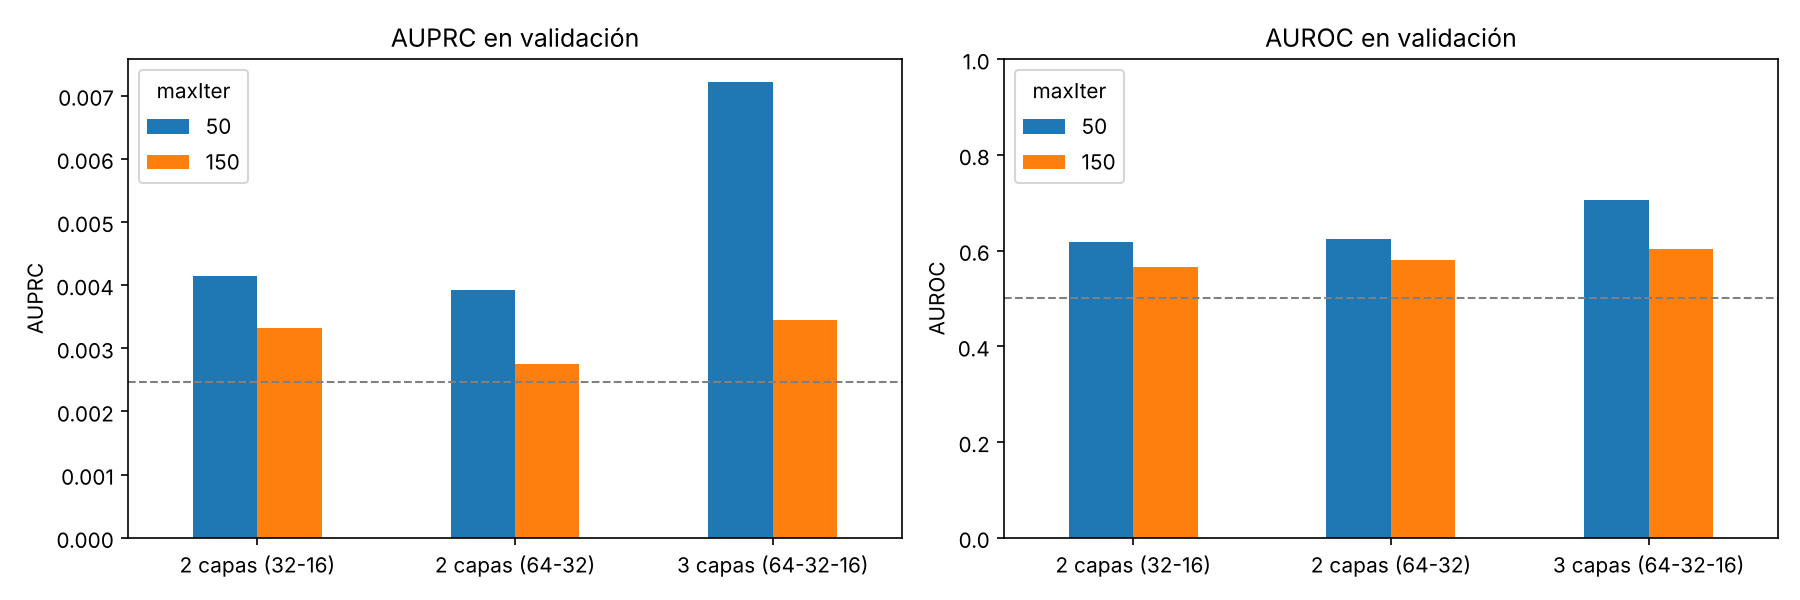
\includegraphics[width=0.95\textwidth]{imagenes/fig_mlp_validacion.png}
    \caption{AUPRC y AUROC en validación (2025) por arquitectura y número de iteraciones. La línea punteada indica la prevalencia base (izquierda) y el nivel de azar $0.5$ (derecha).}
    \label{fig:mlp_validacion}
\end{figure}

\noindent \textbf{Análisis del comportamiento en validación (efecto de parada temprana):}
La arquitectura más profunda de \textbf{tres capas ocultas ($64\text{--}32\text{--}16$) con $50$ iteraciones} alcanzó el mejor desempeño tanto en AUPRC ($0.00721$, casi tres veces la prevalencia base) como en AUROC ($0.7052$). Un hallazgo experimental muy relevante es que, en las tres arquitecturas evaluadas, aumentar las iteraciones de $50$ a $150$ degradó sistemáticamente las métricas de validación: dado que los $219$ casos fatales fueron replicados $381$ veces para equilibrar las clases, prolongar la optimización L-BFGS hace que la red memorice los ejemplos positivos replicados (\textit{overfitting}) y pierda capacidad de generalización sobre el año siguiente. En consecuencia, limitar el entrenamiento a $50$ iteraciones actúa como un mecanismo efectivo de regularización por parada temprana (\textit{early stopping}). Al calibrar el umbral de decisión sobre validación para la red $64\text{--}32\text{--}16$ ($\texttt{maxIter}=50$), el puntaje F1 se maximizó en $\tau = 0.85$.

\subsection{Evaluación Comparativa en Prueba frente a la Regresión Logística}
\label{subsec:bono_dl_comparacion}

La Tabla \ref{tab:mlp_vs_lr_test} y la Figura \ref{fig:mlp_vs_lr_test} comparan el desempeño de la Regresión Logística ($\texttt{regParam}=1.00, \tau=0.55$) y de la Red Neuronal Profunda MLP ($64\text{--}32\text{--}16, \texttt{maxIter}=50, \tau=0.85$) sobre el conjunto de prueba independiente del primer semestre de 2026 ($40,373$ colisiones, $102$ fatales, prevalencia del $0.25\%$).

\begin{table}[H]
\centering
\scriptsize
\renewcommand{\arraystretch}{1.25}
\caption{Comparación en el conjunto de prueba temporal (primer semestre de 2026, prevalencia de $0.25\%$) entre la Regresión Logística y la Red Neuronal Profunda (MLP).}
\label{tab:mlp_vs_lr_test}
\resizebox{\textwidth}{!}{%
\begin{tabular}{l c r r c r r r r}
\toprule
\textbf{Modelo en Spark MLlib} & \textbf{Umbral ($\tau$)} & \textbf{AUPRC} & \textbf{AUROC} & \textbf{Fatales detectadas} & \textbf{Falsos positivos} & \textbf{Precisión} & \textbf{Exhaustividad} & \textbf{F1} \\
\midrule
Regresión Logística & $0.55$ & $0.0042$ & $0.5397$ & $50\text{ de }102$ & $16,382$ & $0.30\%$ & $\mathbf{49.02\%}$ & $0.0060$ \\
\textbf{Red Neuronal (MLP 64--32--16)} & $\mathbf{0.85}$ & $\mathbf{0.0044}$ & $\mathbf{0.6020}$ & $23\text{ de }102$ & $\mathbf{5,934}$ & $\mathbf{0.39\%}$ & $22.55\%$ & $\mathbf{0.0076}$ \\
\bottomrule
\end{tabular}%
}
\end{table}

\begin{figure}[H]
    \centering
    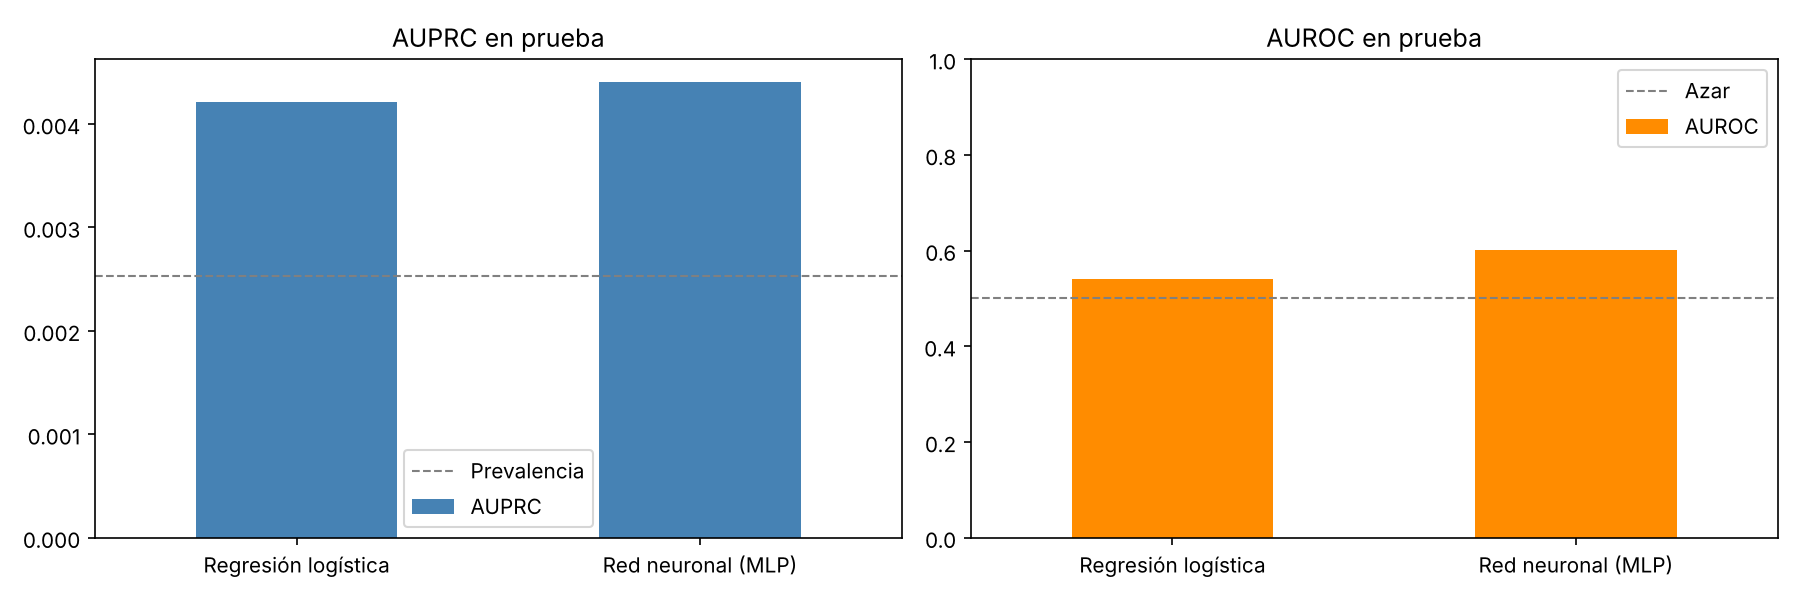
\includegraphics[width=0.95\textwidth]{imagenes/fig_mlp_vs_logistica.png}
    \caption{Comparación de AUPRC (izquierda) y AUROC (derecha) en el conjunto de prueba (2026-I) entre la Regresión Logística y la Red Neuronal (MLP).}
    \label{fig:mlp_vs_lr_test}
\end{figure}

\noindent \textbf{Conclusión del experimento de Aprendizaje Profundo:}
El Perceptrón Multicapa ordenó significativamente mejor las colisiones según su nivel de riesgo letal, elevando el \textbf{AUROC en prueba de $0.5397$ a $0.6020$ ($+6.23$ puntos porcentuales)}, mejorando la \textbf{AUPRC a $0.0044$}, incrementando la \textbf{precisión en un $30\%$ relativo ($0.39\%$ vs. $0.30\%$)} y alcanzando un mayor \textbf{F1 ($0.0076$ vs. $0.0060$)}. Con su umbral calibrado ($\tau = 0.85$), la red neuronal redujo en un \textbf{$63.8\%$ las falsas alarmas} ($5,934$ falsos positivos frente a $16,382$ de la Regresión Logística), a cambio de una menor exhaustividad puntual ($22.55\%$). Esto confirma empíricamente que existen interacciones no lineales entre hora, coordenadas, vehículo y factor contribuyente que las capas ocultas logran extraer, si bien para un sistema de despacho automático de emergencias en tiempo real sería indispensable enriquecer los registros del NYPD/DOT con variables cinemáticas de velocidad e infraestructura vial.
